
% Tento soubor slouží jako šablona/příklad pro generování protokolu

\documentclass{protokol}

%====== Vyplňte údaje ======
\jmeno{David Strašák}
\kod{219502}
\rocnik{3.}
\obor{MET}
% \skupina{3.}
% \spolupracoval{Šimon Pokorný, Bence Simonics}

\merenodne{06.\,03.\,2025}
\odevzdanodne{07\,.03.\,2025}

\nazev{Provedení zkoušek nakrátko a naprázdno na neznámém transformátoru}
% \cislo{99} %měřené úlohy

\predmet{Elektromechanická přeměna energie}
\ustav{UVEE, FEKT VUT v Brně}
% \skola{FEKT VUT v Brně}
%%%%%%%%%%%%%%%%%%%%%%%%%%%%%%%%%%%%%%%%%%%%%%%%%%%%%%%%%%%%%%%%%%%%%%%%%%%%%%%%%%%%%%%%%%%%%%%%%
\begin{document}
%====== Vygenerování tabulky ======
\maketitle
%====== Úvodní texty protokolu ======

\section{Zadání}
\begin{enumerate}
    \item Voltampérovou metodou změřte odpory všech vinutí.
    \item Změřte převod transformátoru.
    \item Proveďte měření nakrátko.
    \item Proveďte měření naprázdno.
    \item Vypočítejte procentní proud naprázdno a procentní napětí nakrátko.
    \item Určete velikosti prvků náhradního schématu transformátoru přepočtené na primární i na sekundární stranu.
    \item Nakreslete dvě náhradní schémata, do jednoho vepište velikosti prvků přepočtené na primární stranu, do druhého na sekundární.
    \item Zhodnoťte měření.
\end{enumerate}

\section{Teoretický rozbor}
Transformátor je netočivý elektrický stroj, který převádí elektrickou energii na elektrickou energii pomocí elektromagnetické indukce. Transformace je provedena na základě přeměny elektrické energie do magnetické a naopak, díky čemuž je transformátor schopný měnit napětí elektřiny, kterou do něj vkládám. Změna napětí je určena převodem transformátoru. 

V naše případě se jednalo o transformátor třífázový. Na tomhle transformátoru je možné ho zapojit do jakékoliv konfigurace s jakýmkoliv hodinovým úhlem. Zadáním ale bylo zapojení Yy0. Spojení do hvězdy se provádí tak, že se všechny konce na vnitřních stranách fází U,V a W spojí na stejný potenciál.

\begin{figure}[H]
    \centering
    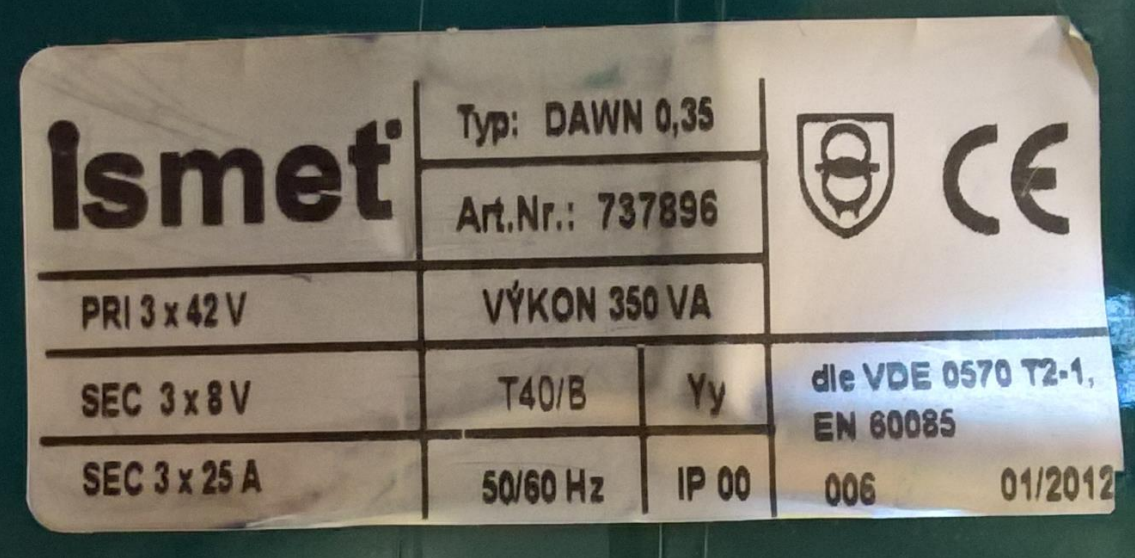
\includegraphics[width=0.8\linewidth]{TrafoStitek.png}
    \caption{Štítek měřeného transformátoru}
    \label{fig:trafoStitek}
\end{figure}

\section{Voltampérovou metodou změřte odpory všech vinutí}
V rámci tohoto úkolu bylo cílem pomocí generátoru stejnosměrného napětí změřit odpor vinutí na jednotlivých fázích transformátoru. 

Postup který byl zvolen v rámci tohoto měření bylo přivést na 1 fázi transformátoru stejnosměrné napětí a změřit napětí a proud na fázi. Následně je pomocí Ohmova zákona možné dopočítat odpor fáze.
\begin{equation}
    R = \frac{U}{I}    
    \label{eq:ohmuvZakon}
\end{equation}

\begin{figure}[H]
    \centering
    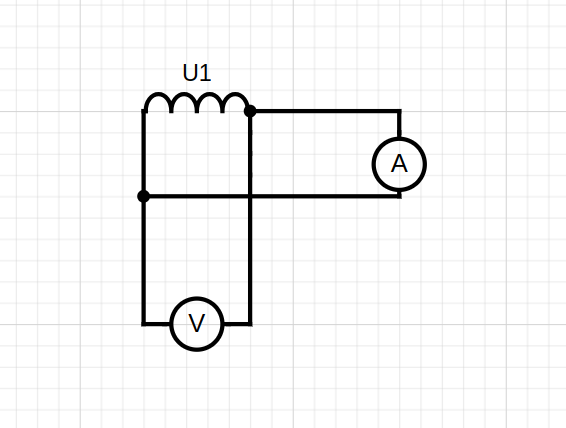
\includegraphics[width=0.5\linewidth]{MereniOdporu.png}
    \caption{Měření odporu na jedné fázi}
    \label{fig:enter-label}
\end{figure}

% Please add the following required packages to your document preamble:
% \usepackage[table,xcdraw]{xcolor}
% Beamer presentation requires \usepackage{colortbl} instead of \usepackage[table,xcdraw]{xcolor}
\begin{table}[H]
\centering
\caption{Měření odporů vinutí transformátoru}
\begin{tabular}{lrrr}
\rowcolor[HTML]{F8F9FA} 
Měření & \multicolumn{1}{l}{\cellcolor[HTML]{F8F9FA}U1{[}V{]}} & \multicolumn{1}{l}{\cellcolor[HTML]{F8F9FA}I1{[}A{]}} & \multicolumn{1}{l}{\cellcolor[HTML]{F8F9FA}Odpor{[}Ohm{]}} \\
\cellcolor[HTML]{FFFFFF}U & \cellcolor[HTML]{FFFFFF}0.722 & 5.268 & 0.137 \\
V & 0.721 & 5.292 & 0.136 \\
W & 0.721 & 5.284 & 0.136 \\
u & 0.272 & 21.923 & 0.012 \\
v & 0.265 & 22.102 & 0.012 \\
w & 0.265 & 22.047 & 0.012
\end{tabular}
\label{tab:MereniOdporuVinuti}
\end{table}

Z tohoto měření vychází průměrné hodnoty odporů vinutí:
\begin{itemize}
    \item $R_{p} = 136 m\Omega$
    \item $R_{s} = 12 m\Omega$
\end{itemize}

\section{Změřte převod transformátoru}
Změřit převod transformátoru je možné tím, že se zároveň měří napětí na jedné fázi primáru a zároveň na stejné fázi sekundáru. Během měření převodu by mělo být na primáru nastavené jmenovité napětí, vzhledem k tomu, že se měří naprázdno. 

Vzhledem k tomu, že jsme měříme fázové napětí, je nejdříve nutné ještě přepočítat jmenovité napětí na fázové. Tohle děláme abychom měli na fázi blízké napětí, které se na fázi objeví během běžného používání transformátoru. Z tohoto se určí jmenovité napětí, které bylo během zkoušky nastavené na primáru transformátoru na hodnotu:

\begin{equation}
    U1f = \frac{U1}{\sqrt{3}} = \frac{42}{\sqrt{3}} = 24,25 V
    \label{eq:PrevodNominalnihoNapetiNaFazove}
\end{equation}

\begin{table}[H]
\centering
\caption{Hodnoty naměřené na primárním a sekundárním vinutí transformátoru}
\begin{tabular}{ll}
\rowcolor[HTML]{F8F9FA} 
U1[V]& U2[V] \\
\rowcolor[HTML]{FFFFFF} 
\multicolumn{1}{r}{\cellcolor[HTML]{FFFFFF}24.233} & \multicolumn{1}{r}{\cellcolor[HTML]{FFFFFF}4.955}
\end{tabular}
\label{tab:NamereniNapetiNaPrimaruASekundaru}
\end{table}

Z těchto hodnot je možné vypočítat převod transformátoru pomocí tohoto vzorce:
\begin{equation}
    k = \frac{U1f}{U2f} = \frac{24.233}{4.955} = 4.891
    \label{eq:vypocetPrevoduTransformatoru}
\end{equation}

\section{Vypočtěte procentní proud naprázdno a procentní napětí nakrátko}
\subsection{Procentní proud naprázdno}
Zkouška naprázdno se provádí na sekundární straně a měří se při nominálním napětí mezi fázemi. Vzhledem k tomu, že si pomocí autotransformátoru nastavujeme napětí, není potřeba počítat proud, protože se změří během zkoušky.

Na sekundární straně se nastaví napětí sekundáru, které je 8V.

\subsection{Procentní napětí nakrátko}

\section{Proveďte měření nakrátko}
\begin{table}[H]
\centering
\caption{Výsledky měření nakrátko}
\label{tab:mereniNakratko}
\begin{tabular}{lllllllll}
\rowcolor[HTML]{F8F9FA} 
U1{[}V{]} & U2{[}V{]} & U3{[}V{]} & U0{[}A{]} & I1{[}A{]} & I2{[}A{]} & I3{[}A{]} & I0{[}A{]} & P0{[}W{]} \\
\rowcolor[HTML]{FFFFFF} 
\multicolumn{1}{r}{\cellcolor[HTML]{FFFFFF}4.820} & \multicolumn{1}{r}{\cellcolor[HTML]{FFFFFF}4.909} & \multicolumn{1}{r}{\cellcolor[HTML]{FFFFFF}4.931} & \multicolumn{1}{r}{\cellcolor[HTML]{FFFFFF}4.886} & \multicolumn{1}{r}{\cellcolor[HTML]{FFFFFF}4.729} & \multicolumn{1}{r}{\cellcolor[HTML]{FFFFFF}4.824} & \multicolumn{1}{r}{\cellcolor[HTML]{FFFFFF}4.707} & \multicolumn{1}{r}{\cellcolor[HTML]{FFFFFF}4.753} & \multicolumn{1}{r}{\cellcolor[HTML]{FFFFFF}40.122}
\end{tabular}
\end{table}

\section{Proveďte měření naprázdno}
\begin{table}[H]
\centering
\caption{Výsledky měření naprázdno}
\label{tab:mereniNaprazdno}
\begin{tabular}{lllllllll}
\rowcolor[HTML]{F8F9FA} 
U1{[}V{]} & U2{[}V{]} & U3{[}V{]} & U0{[}A{]} & I1{[}A{]} & I2{[}A{]} & I3{[}A{]} & I0{[}A{]} & P0{[}W{]} \\
\rowcolor[HTML]{FFFFFF} 
\multicolumn{1}{r}{\cellcolor[HTML]{FFFFFF}7.990} & \multicolumn{1}{r}{\cellcolor[HTML]{FFFFFF}8.134} & \multicolumn{1}{r}{\cellcolor[HTML]{FFFFFF}8.253} & \multicolumn{1}{r}{\cellcolor[HTML]{FFFFFF}8.125} & \multicolumn{1}{r}{\cellcolor[HTML]{FFFFFF}2.742} & \multicolumn{1}{r}{\cellcolor[HTML]{FFFFFF}2.008} & \multicolumn{1}{r}{\cellcolor[HTML]{FFFFFF}2.545} & \multicolumn{1}{r}{\cellcolor[HTML]{FFFFFF}2.432} & \multicolumn{1}{r}{\cellcolor[HTML]{FFFFFF}9.832}
\end{tabular}
\end{table}

\section{Určete velikosti prvků náhradního schématu transformátoru přepočtené na primární
i na sekundární stranu.}

 \section{akreslete dvě náhradní schémata, do jednoho vepište velikosti prvků přepočtené
na primární stranu, do druhého na sekundární.}

\section{Závěr}
\dots




\end{document}